% ─────────────────────────────────────────────────────────────────────────────
\chapter{State of the Art}
\label{chap:state-of-the-art}
% ─────────────────────────────────────────────────────────────────────────────
This chapter examines the scientific literature relevant to the thematic axes
of the thesis, following the editorial distinction established with respect to
Chapter~\ref{chap:background}: for each area, it discusses the main existing
contributions, what they have demonstrated, and which limitations remain open,
without redefining concepts already introduced in the theoretical background.
The objective is to identify the specific gap that motivates the experimental
approach of the thesis: the limited availability, in the existing literature,
of integrated experimental protocols for evaluating the operational robustness
of proxy models and AI-based software in realistic forensic scenarios.


% ─────────────────────────────────────────────────────────────────────────────
\section{AI and Automation in Digital Forensics}
\label{sec:sota-ai-df}
% ─────────────────────────────────────────────────────────────────────────────

The scale of digital data represents the starting point of the literature on
automation in \gls{df}. Garfinkel~\cite{garfinkel2010digital}, in a work that
shaped research over the following decade, documented how the rapid growth of
digital data volumes was making manual analysis increasingly unsustainable,
identifying automation as one of the priority directions for investment. The
contribution did not concern specific solutions, but rather a mapping of
unresolved problems: among them, the lack of methods for the automatic triage
of large multimedia corpora, the absence of shared benchmarks, and the
difficulty of evaluating tools under realistic operational conditions. This
agenda influenced subsequent research, which responded through the progressive
integration of \gls{ml} and \gls{dl} techniques into forensic workflows.

A first systematic attempt to map this integration was provided by Marturana et
al.~\cite{marturana2011digital}, who analyzed the state of the art of
artificial intelligence applied to \gls{df} at a time when the field was still
predominantly experimental. Their work showed that existing applications were
fragmented across domains---file system analysis, content classification, and
pattern matching---and that a unified approach capable of covering the entire
investigative workflow was lacking. The models proposed in the literature
achieved good performance in controlled settings, but had not been
systematically evaluated on data originating from real-world scenarios or
tested with respect to their reliability in the presence of anomalous inputs.

This research direction consolidated over the following decade. Costantini et
al.~\cite{costantini2019digital} proposed a framework integrating automated
reasoning and \gls{ml} techniques to support the forensic analyst in managing
complex evidence, with applications to event correlation and multimedia content
classification. The work documents how \gls{ai} can reduce the operational
workload in the examination and analysis phases, but leaves the issue of
robustness open: the framework assumes well-formed data and does not address
scenarios in which inputs have been manipulated or degraded. This limitation is
relevant because real forensic data are often of variable quality and may have
been intentionally altered before acquisition.

A more recent and operationally oriented perspective is provided by
Faqir~\cite{faqir2023digital}, who offers an overview of \gls{ai}-based
applications in contemporary digital investigations, including automatic
triage, classification of illicit content, facial recognition, and
communication analysis. The work highlights that the adoption of these tools in
investigative practices has grown significantly, but also emphasizes a still
unresolved tension: most systems are evaluated in terms of aggregate accuracy
on controlled datasets, without adequately considering the stability of their
predictions under manipulated or out-of-distribution input conditions. This gap
between performance measured under controlled conditions and operational
reliability is one of the most relevant critical points for positioning the
present thesis.

A more recent perspective broadens the operational framework by jointly
considering the opportunities offered by \gls{ai} in digital investigations and
the risks arising from its possible use for evasive or anti-forensic purposes.
Along these lines, Sanna et al.~\cite{sanna2025cybercrime} discuss the possible
support provided by \gls{ai} to cybercrime detection and \gls{df} activities,
while also highlighting how general-purpose generative tools may facilitate the
production of images or code intended for the steganographic concealment of
information. The empirical evaluation of the robustness of AI-based software
with respect to manipulated visual content is instead addressed more directly
by the studies on \textit{Magnet.AI} and \textit{Excire Photo AI}, discussed in
the following section \cite{sanna2024preliminary,sanna2025pixelperfect}.

Overall, this line of research has produced three consolidated findings. First,
\gls{ai}-based automation in \gls{df} is motivated by a real problem of scale
that traditional methods can no longer manage in a fully sustainable way
\cite{garfinkel2010digital,costantini2019digital}. Second, \gls{ai} acts as an
operational support for the analyst, not as a substitute, and evidentiary
conclusions remain a human responsibility
\cite{faqir2023digital,sanna2025cybercrime}. Third, the validation of
\gls{ai}-based systems in \gls{df} remains partial: the literature tends to
test models on clean and controlled data, while less systematically studying
their behavior when inputs are degraded, manipulated, or out of distribution
\cite{sanna2024preliminary,sanna2025pixelperfect}.

It is precisely this third point that opens the specific problem addressed in
the following section: if the validation of \gls{ai}-based models in \gls{df}
is still incomplete at the academic level, the situation becomes even more
critical for commercial software used or evaluated in the context of forensic
analysis, where \gls{ai}-based functionalities may be proprietary, opaque, and
difficult to subject to independent verification.


% ─────────────────────────────────────────────────────────────────────────────
\section{AI-based Software for Forensic Image Analysis and Operational Validation}
\label{sec:sota-ai-tools}
% ─────────────────────────────────────────────────────────────────────────────
The integration of \gls{ai}-based functionalities into software used for the
analysis of digital evidence represents one of the main operational evolutions
of \gls{df}. In the case of visual content, such functionalities can support
triage, semantic search, automatic categorization, and the prioritization of
images to be submitted to analyst review. However, the availability of an
automated function does not, in itself, imply that its behavior is sufficiently
robust in the presence of degraded, ambiguous, or intentionally manipulated
inputs. This problem is particularly relevant when AI components are
proprietary and the software can be observed only through its produced outputs,
without access to the internal models, training datasets, or decision thresholds
adopted \cite{costantini2019digital,sanna2024preliminary,sanna2025pixelperfect}.

The literature specifically devoted to the operational robustness of AI-based
software usable in forensic contexts remains limited. Sanna et al.\ conducted
an initial analysis of \textit{Magnet.AI}, integrated into \textit{Magnet
AXIOM}, and \textit{Excire Photo AI}, examining the behavior of automatic
functionalities with respect to anomalous or manipulated content
\cite{sanna2024preliminary}. A subsequent study further investigated the
response of the same software to facial deepfakes and morphed images,
identifying critical issues in the robustness of the analyzed AI-enhanced
functionalities and emphasizing the particular forensic relevance of false
negatives, since potentially relevant content may fail to be brought to the
analyst's attention \cite{sanna2025pixelperfect}. These works constitute the
closest reference to the present thesis, while differing from the problem
considered here, which concerns the operational \texttt{weapon}/\texttt{non\_weapon}
task, oriented toward the identification of images containing firearms or
firearm-oriented content, and the separate analysis of system behavior in the
presence of \texttt{ood} content.

% ─────────────────────────────────────────────────────────────────────────────
\subsection{Magnet AXIOM and Magnet.AI}
\label{subsec:sota_magnet_ai}
% ─────────────────────────────────────────────────────────────────────────────
\textit{Magnet AXIOM} is commercial software designed for the processing and
analysis of evidence originating from heterogeneous digital sources. Among the
functionalities relevant to automated image analysis, the \textit{Magnet.AI}
component makes it possible to categorize multimedia content that may be
relevant to an investigation, including categories related to weapons, drugs,
nudity, and other sensitive content \cite{magnetai_official,sanna2024preliminary}.
This functionality is directly relevant to the task addressed in the present
thesis, because it makes it possible to observe whether images containing
firearms or firearm-oriented content are flagged within a forensic analysis
workflow.

Previous studies have shown that \textit{Magnet.AI} can be subjected to
operational evaluation in a \textit{black-box} setting, by observing the
categories returned by the software without assuming knowledge of the
underlying model. In particular, Sanna et al.\ examined the behavior of the
software with respect to manipulated content and, subsequently, with respect to
facial images generated through deepfake and morphing techniques, identifying
limitations in the robustness of some automatic functionalities
\cite{sanna2024preliminary,sanna2025pixelperfect}. The main methodological
limitation remains the opacity of the proprietary component: the researcher can
measure the behavior of the outputs available to the analyst, but cannot
reconstruct with certainty the architecture, training data, pre-processing, or
internal decision logic.

% ─────────────────────────────────────────────────────────────────────────────
\subsection{Excire Foto 2025}
\label{subsec:sota_excire_foto}
% ─────────────────────────────────────────────────────────────────────────────
Previous literature has analyzed \textit{Excire Photo AI} as AI-based software
oriented toward the search and recognition of photographic content, including
in controlled forensic analysis contexts
\cite{sanna2024preliminary,sanna2025pixelperfect}. In these studies, Excire was
evaluated primarily with respect to identity search functionalities and its
behavior on manipulated facial images. The reported results show that deepfakes
and morphing can substantially degrade the reliability of automatic image
retrieval associated with specific identities \cite{sanna2025pixelperfect}.

The scope of the present thesis is different. The software considered is
\textit{Excire Foto 2025}, used as a standalone general-purpose application
equipped with AI functionalities for organizing and searching visual content,
and not as a native component of a tool developed exclusively for forensic
purposes \cite{excirefoto2025_official}. Its inclusion in the study responds to
the methodological interest in verifying whether a visual semantic search
system can be used, in a controlled forensic analysis context, to retrieve
images consistent with an investigatively relevant concept such as the presence
of a weapon.

This distinction is essential for interpreting the results: \textit{Excire Foto
2025} should not be described as a native forensic
\texttt{weapon}/\texttt{non\_weapon} classifier, but rather as AI-based software
whose observable behavior can be mapped to an operational decision of retrieval
or non-retrieval of an image with respect to the queries and configurations
defined in the experimental protocol. In this case as well, the evaluation
remains \textit{black-box}: the thesis measures the outputs available to the
analyst, without assuming knowledge of the model, the training data, or the
internal similarity criteria.

% ─────────────────────────────────────────────────────────────────────────────
\subsection{Cellebrite Inseyets and Automated Media Classification}
\label{subsec:sota_cellebrite}
% ─────────────────────────────────────────────────────────────────────────────
The Cellebrite ecosystem is widely associated with mobile forensics and digital
investigation activities. The vendor documentation describes \textit{Cellebrite
Inseyets} as an integrated suite for accessing, extracting, processing,
analyzing, and reporting on digital evidence originating primarily from mobile
devices \cite{cellebrite_inseyets_official}. From this perspective, Inseyets
does not represent a single isolated module, but an operational environment
that combines extraction, analysis, triage, and investigative workflow
management functionalities.

With respect to visual content, Cellebrite documentation also describes
\textit{media classification} functionalities oriented toward the automated
categorization of images and videos through AI-based techniques
\cite{cellebrite}. These functionalities are part of a broader trend in
contemporary Digital Forensics, in which commercial tools integrate automatic
modules to support the triage, selection, and prioritization of large volumes
of multimedia content.

In the context of the present thesis, \textit{Cellebrite Inseyets} is therefore
relevant as an example of commercial black-box software in which AI-assisted
functionalities are integrated into professional mobile forensic analysis
workflows. Compared with desktop or general-purpose tools primarily oriented
toward photographic search and categorization, Cellebrite makes it possible to
extend the reasoning on operational robustness to a context closer to mobile
forensics, where the analyst may need to examine large volumes of images and
videos extracted from devices or digital storage media.

As with the other commercial tools considered in the state of the art, the
integration of automatic functionalities does not eliminate the need to assess
their reliability, limitations, and behavior in the presence of degraded,
manipulated, or not fully representative inputs with respect to ideal operating
conditions. For this reason, Cellebrite Inseyets is recalled as a further
significant case of commercial black-box software with respect to the general
problem of the operational robustness of AI-assisted systems in forensic
contexts.
% ─────────────────────────────────────────────────────────────────────────────
\subsection{Magnet Griffeye e T3K CORE}
\label{subsec:sota_griffeye_t3k}
% ─────────────────────────────────────────────────────────────────────────────
\textit{Magnet Griffeye} is a commercial platform used for the triage, review,
and organization of large volumes of multimedia content in investigative and
forensic contexts. In the context of the present thesis, the tool is relevant
not as a controllable academic classifier, but as commercial black-box software
capable of producing observable semantic outputs on images through automatic
analysis modules.

The \textit{T3K CORE} component makes it possible to generate automatic
semantic bookmarks associated with the analyzed multimedia content. These
bookmarks can be used by the analyst to filter, prioritize, or review
potentially relevant images. From a methodological perspective, this type of
output differs from the categories returned by \textit{Magnet.AI}, from the
semantic retrieval results produced by \textit{Excire Foto 2025}, and from the
classifications exported in the Cellebrite workflow. Nevertheless, it belongs
to the same family of observable operational signals that can be normalized
against an experimental ground truth.

The relevance of \textit{Magnet Griffeye} for this thesis therefore lies in the
possibility of extending the black-box evaluation to an additional output
paradigm: not a class probability or an explicit supervised decision, but a set
of automatically generated semantic bookmarks. This characteristic reinforces
the general methodological problem addressed in the thesis: different
commercial tools may expose heterogeneous outputs, but they must be mapped to a
common representation only through explicit, documented rules for normalization
that are consistent with the experimental task.


% ─────────────────────────────────────────────────────────────────────────────
\subsection{Common Limitations of Black-Box Evaluation}
\label{subsec:sota_black_box_limits}
% ─────────────────────────────────────────────────────────────────────────────
The software considered presents different functional characteristics and
should not be interpreted as directly equivalent systems. \textit{Magnet.AI}
exposes operational categories applicable to image content; \textit{Excire Foto
2025} is considered as a system for semantic search and retrieval of visual
content; \textit{Cellebrite Inseyets} requires the identification of the
component concretely used for media categorization; \textit{Magnet Griffeye},
through \textit{T3K CORE}, produces automatic semantic bookmarks. Therefore, an
operational comparison among these software systems cannot presuppose identity
of task, internal models, decision thresholds, or output modalities.

A common limitation concerns the proprietary or otherwise non-observable nature
of the AI components employed. In a \textit{black-box} evaluation, it is not
possible to directly control the model architecture, training dataset, update
procedures, pre-processing, confidence calibration, or decision criteria.
Validation must therefore rely on external and verifiable elements:
independent ground truth, a documented dataset, common experimental conditions,
reproducible manipulated inputs, exportable outputs, and matching procedures
based on identifiers or hashes.

In light of these limitations, the contribution of the present thesis does not
consist in internally characterizing the proprietary algorithms of the software
analyzed, nor in proposing a new classification tool. Rather, it consists in
evaluating, through a reproducible experimental protocol, the operational
robustness of observable outputs in the presence of clean images,
out-of-distribution content, adversarial perturbations, and anti-forensic
transformations. This setting extends previous literature toward a different
visual task of investigative interest and toward a comparison between
controllable proxy models and AI-based software evaluated in a \textit{black-box}
setting.

\begin{table}[htbp]
    \centering
    \small
    \renewcommand{\arraystretch}{1.25}
    \begin{tabularx}{\textwidth}{@{}p{2.8cm}p{3.5cm}X p{3.2cm}@{}}
        \toprule
        \textbf{Software} &
        \textbf{Relevant function} &
        \textbf{Relevance to the present thesis} &
        \textbf{Methodological limitation} \\
        \midrule
        Magnet AXIOM / Magnet.AI &
        Automated categorization of visual content, including images associated with weapons &
        Makes it possible to observe the operational flagging of \texttt{weapon} images in software designed for forensic analysis &
        Proprietary AI component evaluable only through observable outputs \\
        \addlinespace
        Excire Foto 2025 &
        AI-assisted semantic search and retrieval of images &
        Makes it possible to evaluate the retrieval of images consistent with the firearm-oriented concept through standalone software evaluated in a controlled forensic context &
        Not a native forensic classifier; behavior depends on operational queries and configurations \\
        \addlinespace
        Cellebrite Inseyets &
        AI-assisted categorization of images and videos within mobile analysis &
        Makes it possible to verify the applicability of the bundle to a mobile analysis workflow, based on the outputs concretely exportable from the software &
        Commercial black-box tool; comparability depends on the format of exportable outputs and on the operational recoding of classifications \\
        \addlinespace
        Magnet Griffeye / T3K CORE &
        Automatic generation of semantic bookmarks on multimedia content &
        Makes it possible to evaluate an additional black-box output paradigm, based on semantic bookmarks that can be normalized with respect to the experimental task &
        Commercial black-box tool; comparability depends on the operational mapping between exported bookmarks and the experimental \texttt{weapon} class \\
        \addlinespace
        \bottomrule
    \end{tabularx}
    \caption{AI-based software relevant to the operational evaluation and main limitations of their black-box analysis.}
    \label{tab:sota_ai_based_software}
\end{table}


% ─────────────────────────────────────────────────────────────────────────────
\section{Automated Image Classification in Forensic Scenarios}
\label{sec:sota-image-classification}
% ─────────────────────────────────────────────────────────────────────────────

Automated image classification constitutes one of the main points of contact
between computer vision and \gls{df}. In the forensic literature, the problem
is not addressed as a simple general visual recognition task, but as an
activity supporting the selection and prioritization of potentially relevant
evidence within large multimedia collections. In this context, the objective is
not only to assign a correct label to an image, but also to reduce the
analyst's workload, increase the likelihood of identifying investigatively
significant content, and limit the risk that relevant elements remain hidden
within very large datasets~\cite{costantini2019digital,sanna2024preliminary}.

Early contributions in this direction applied \gls{ml} and \gls{dl} models to
semantic classification, object recognition, and multimedia triage tasks, with
particular attention to categories of investigative interest such as faces,
objects, scenes, illicit content, or elements potentially associated with
criminal conduct. Costantini et al.~\cite{costantini2019digital} place these
functionalities within a broader evidence analysis workflow, in which automated
classification does not replace forensic interpretation, but contributes to
organizing and filtering the acquired material. This setting is relevant
because it clarifies that visual classification, in forensic contexts, has a
primarily operational function: directing the analyst's attention toward
portions of evidence that deserve more detailed review.

In the specific domain of weapon recognition, Hao et al.~\cite{Hao2018DeepFirearm}
proposed DeepFirearm, an approach based on deep representations for
fine-grained firearm recognition. Their contribution shows that the
classification of images containing firearms or firearm-oriented content cannot
be reduced to a trivial visual problem: the variability of poses, perspectives,
occlusions, image quality, and morphological similarity among different models
requires discriminative representations capable of capturing relevant visual
details. However, works of this type are mainly oriented toward recognition or
retrieval under controlled experimental conditions, and do not systematically
address the behavior of models when images are degraded, manipulated, or
originating from heterogeneous sources typical of a digital investigation.

The availability of public datasets for weapon detection, such as the
\textit{Weapon Detection Dataset}~\cite{Sanyal2023KaggleWeapon}, has supported
the development of models capable of recognizing firearms or firearm-oriented
content in static images. These resources have important experimental value,
but present limitations when transferred to realistic forensic scenarios.
Public datasets are often designed for visual recognition or surveillance
applications, rather than for the operational validation of AI-based models and
software usable in forensic contexts. As a result, they may not adequately
represent borderline cases, degraded images, out-of-distribution content,
screenshots, synthetic images, or material originating from social platforms
and messaging applications. This distance between benchmark datasets and real
investigative material constitutes one of the most relevant critical issues in
the evaluation of \gls{ai}-based systems applied to \gls{df}.

From an architectural perspective, the computer vision literature has shown the
effectiveness of deep \gls{cnn} architectures for image classification.
Architectures such as ResNet~\cite{he2016deep} and
EfficientNet~\cite{tan2019efficientnet} have provided solid foundations for
many visual classification systems, owing to their ability to learn
hierarchical representations of image content. More recently, vision-language
models such as \gls{clip}~\cite{radford2021learning} and
\gls{blip}~\cite{li2022blip}, together with \gls{vit} architectures
\cite{dosovitskiy2020image}, have broadened the scope of automated
classification by enabling forms of text-guided, zero-shot, or
semantic-description-based classification. In forensic contexts, this evolution
is potentially relevant because investigative categories may not perfectly
coincide with the classes of traditional datasets; however, the literature has
not yet sufficiently clarified how stable these models are in the presence of
degraded, ambiguous, or manipulated images.

A recurring aspect in the literature is the different operational severity of
classification errors. In forensic tasks, a false positive may increase the
analyst's review burden, but a false negative may prevent relevant content from
being submitted to human review. This asymmetry is particularly important in
triage systems, in which the automatic output does not directly produce an
evidentiary conclusion, but influences the order in which evidence is examined.
Consequently, the evaluation of a forensic classifier cannot be limited to
average accuracy: it must also consider recall on critical investigative
classes, the distribution of errors, the stability of predictions, and the
ability not to assign a known class with excessive confidence to
out-of-distribution inputs.

The most recent literature on AI-based software usable in forensic contexts
confirms this critical issue. Sanna et al.~\cite{sanna2024preliminary} show
that automatic classification functionalities integrated into operational
software may produce unstable results when visual content deviates from
expected conditions. Although these studies do not exhaust the problem of image
classification in forensic contexts, they clearly indicate that the transition
from models that are accurate on controlled datasets to tools that are reliable
in investigative scenarios requires more rigorous evaluation protocols. In
particular, the combination of visual classification, investigatively relevant
content, out-of-distribution images, and intentional manipulations remains
poorly explored.

Overall, the literature on automated image classification provides useful
models and datasets, but leaves open a specific problem for \gls{df}: the
limited availability of integrated evaluations that simultaneously consider the
investigative relevance of the classes, the heterogeneity of sources, the
presence of borderline or \gls{ood} cases, and robustness with respect to
degradations, anti-forensic manipulations, or adversarial perturbations. This
gap prepares the transition to the following section, devoted to benchmarks and
results from the literature on the robustness of computer vision models.




% ─────────────────────────────────────────────────────────────────────────────
\section{Adversarial Machine Learning applicato a classificatori di immagini}
\label{sec:sota-adversarial-ml}
% ─────────────────────────────────────────────────────────────────────────────

La letteratura sull'\gls{advml} ha mostrato che i classificatori di immagini
basati su \gls{ml} e \gls{dl} possono essere vulnerabili a input costruiti
intenzionalmente per alterarne la predizione. Nel
Capitolo~\ref{chap:background} sono stati introdotti i concetti fondamentali di
adversarial example, threat model e perturbazione dell'input; in questa sezione
l'attenzione è invece rivolta ai principali risultati della letteratura e alla
loro rilevanza per i classificatori visuali impiegabili in scenari forensi.

I lavori seminali di Szegedy et al.~\cite{szegedy2014intriguing} e Goodfellow
et al.~\cite{goodfellow2015explaining} hanno stabilito che classificatori
profondi ad alta accuratezza possono produrre decisioni errate in presenza di
perturbazioni intenzionalmente costruite, anche quando tali alterazioni risultano
limitate sul piano percettivo. Per la \gls{df}, questo risultato è rilevante
perché mostra che un sistema automatico impiegato nel triage visuale può essere
indotto a sottostimare o ignorare contenuti investigativamente rilevanti qualora
l'input sia stato manipolato prima dell'acquisizione o dell'analisi.

Un secondo filone della letteratura ha approfondito la costruzione di attacchi
più precisi, iterativi o ottimizzati rispetto alla minima perturbazione
necessaria per modificare la decisione del modello. DeepFool
\cite{moosavi2016deepfool} ha mostrato che è possibile stimare perturbazioni di
piccola ampiezza capaci di spostare l'immagine oltre il confine decisionale del
classificatore, contribuendo a rendere più sistematica la valutazione della
distanza tra input pulito e input adversariale. \gls{superdeepfool}
\cite{zhang2024superdeepfool} si colloca nello stesso filone, proponendo
un'evoluzione orientata a generare perturbazioni efficaci rispetto a modelli
profondi con un processo di ottimizzazione più mirato. Questi lavori non sono
nati specificamente per la \gls{df}, ma sono rilevanti perché forniscono una
base metodologica per misurare quanto un classificatore visuale possa essere
instabile rispetto a variazioni non casuali dell'immagine.

La letteratura ha inoltre mostrato che la vulnerabilità adversariale non
riguarda soltanto perturbazioni distribuite su molti pixel. Su et
al.~\cite{su2019onepixel} hanno introdotto il \gls{onepixel}, dimostrando che,
in alcuni casi, la modifica di un numero estremamente limitato di pixel può
essere sufficiente a indurre una classificazione errata. Più recentemente,
approcci basati su vincoli sparsi, come \gls{sigmazero}
\cite{zhao2024sigmazero}, hanno ulteriormente esplorato la possibilità di
costruire attacchi con alterazioni localizzate e ridotto impatto percettivo.
Questa linea di ricerca è particolarmente significativa per il contesto forense,
perché mostra che la manipolazione efficace di un'immagine non richiede
necessariamente trasformazioni estese o visivamente evidenti: anche modifiche
localizzate possono interferire con il comportamento di modelli automatici.

Un'ulteriore linea di ricerca ha mostrato che la perturbazione adversariale può
assumere anche forme localizzate e visivamente più esplicite, come nel caso
degli adversarial patch. Brown et al.~\cite{brown2017patch} hanno dimostrato
che una regione artificiale applicata all'immagine può indurre errori di
classificazione anche senza modificare l'intero contenuto visivo. Per la
presente tesi, tale risultato è rilevante soprattutto sul piano concettuale:
mostra che la vulnerabilità dei classificatori non riguarda soltanto
perturbazioni distribuite e quasi impercettibili, ma anche alterazioni
localizzate che possono interferire con il processo decisionale del modello.

La letteratura comprende inoltre attacchi generativi, nei quali reti generative
vengono addestrate per produrre perturbazioni adversariali trasferibili. Un
esempio rappresentativo è AdvGAN, che impiega un generatore per costruire esempi
adversariali in modo efficiente e con capacità di trasferimento tra modelli
\cite{xia2018advgan}. Questa famiglia di attacchi non è inclusa nel protocollo
sperimentale della presente tesi, poiché il lavoro privilegia perturbazioni più
direttamente interpretabili nel contesto operativo della \gls{df}.

Un aspetto cruciale per gli scenari operativi è la distinzione tra attacchi
white-box, black-box e transfer-based. Papernot et
al.~\cite{papernot2016limitations} hanno mostrato che la vulnerabilità dei
modelli può trasferirsi tra classificatori differenti, mentre la letteratura
successiva sugli attacchi black-box ha sistematizzato scenari nei quali
l'attaccante dispone soltanto di accesso limitato agli output del modello o
utilizza modelli surrogati per generare perturbazioni trasferibili
\cite{bhambri2020survey}. Carlini e Wagner~\cite{carlini2017towards} hanno
contribuito a rafforzare la valutazione della sicurezza dei classificatori
mostrando i limiti di diverse difese proposte contro gli attacchi
adversariali. Le survey di Akhtar e Mian~\cite{akhtar2018threat} e Yuan et
al.~\cite{yuan2019adversarial} confermano che la trasferibilità degli
adversarial examples costituisce uno dei problemi più rilevanti per l'impiego di
modelli \gls{ai}-based in ambienti non completamente controllati. Nel caso dei
software commerciali valutati in contesto forense, questa osservazione assume
particolare importanza: anche quando il modello integrato nel software è
proprietario e non ispezionabile, un attaccante potrebbe generare perturbazioni
su modelli accessibili e verificarne l'efficacia per trasferimento.

Biggio e Roli~\cite{biggio2018wild} hanno inquadrato queste vulnerabilità
all'interno del paradigma dell'\textit{adversary-aware security}, sostenendo che
la valutazione di un sistema basato su apprendimento automatico deve considerare
esplicitamente la presenza di un avversario strategico. Questo principio è
centrale per la presente tesi: un sistema di classificazione forense non opera
necessariamente in un ambiente neutro, ma può essere esposto a dati preparati o
modificati da soggetti interessati a ostacolare l'analisi. La robustezza
adversariale, quindi, non è soltanto una proprietà tecnica del modello, ma una
componente della sua affidabilità operativa.

Nel dominio più vicino all'image forensics, Barni et al.~\cite{barni2018cf}
hanno mostrato che modelli basati su reti neurali per la rilevazione di
manipolazioni digitali possono essere vulnerabili ad attacchi adversariali.
Nowroozi~\cite{nowroozi2020phd} ha ulteriormente approfondito il problema delle
tecniche di \gls{ml} per l'image forensics in scenari adversariali,
evidenziando come modelli progettati per analisi forensi possano essere
degradati da perturbazioni mirate. Questi contributi sono particolarmente
importanti perché spostano il problema dagli esempi generici di computer vision
ai sistemi utilizzati per compiti più vicini al dominio forense. Il risultato
che emerge è che la vulnerabilità adversariale non riguarda soltanto
classificatori generici addestrati su dataset standard, ma anche modelli
sviluppati per riconoscere manipolazioni o caratteristiche rilevanti in immagini
digitali.

Il collegamento con i software \gls{ai}-based utilizzabili in contesti forensi è
stato rafforzato dai lavori più recenti sulla robustezza operativa. Nowroozi et
al.~\cite{nowroozi2024verifying} hanno mostrato, in un diverso contesto di
sicurezza, che la verifica della robustezza rispetto a perturbazioni
adversariali deve essere parte integrante della valutazione dei sistemi
automatici. Sanna et al.~\cite{sanna2024preliminary,sanna2025pixelperfect}
hanno portato questa prospettiva più direttamente nel dominio dell'analisi
forense, evidenziando che funzionalità \gls{ai}-based integrate in software
operativi possono mostrare fragilità quando esposte a contenuti manipolati.
Sebbene tali studi non esauriscano l'intero spettro degli attacchi adversariali
su immagini, indicano con chiarezza che la validazione dei software
\gls{ai}-based utilizzabili in contesti forensi non può limitarsi alla loro
efficacia su input ordinari.

Un ulteriore filone della letteratura ha analizzato l'uso di trasformazioni
sull'input come possibile difesa rispetto agli esempi adversariali. Tecniche
quali ricompressione, ridimensionamento o trasformazioni dell'immagine possono
ridurre l'efficacia di alcune perturbazioni, ma non eliminano il problema della
valutazione sistematica della robustezza \cite{guo2017countering}. Questo
aspetto è rilevante per la presente tesi perché alcune trasformazioni considerate
nella letteratura come meccanismi di difesa possono assumere, in un contesto
forense, un significato diverso: non sono impiegate per proteggere il modello,
ma per simulare condizioni di stress anti-forense realistiche e valutare la
stabilità operativa dei classificatori e degli strumenti commerciali.

Nel complesso, la letteratura sull'\gls{advml} applicato alle immagini fornisce
tre indicazioni rilevanti per questa tesi. In primo luogo, i classificatori
visuali possono essere vulnerabili a perturbazioni intenzionali anche quando
presentano prestazioni elevate su dati puliti. In secondo luogo, tale
vulnerabilità può manifestarsi in scenari diversi per conoscenza
dell'attaccante, ampiezza della perturbazione e trasferibilità tra modelli. In
terzo luogo, i lavori specifici sull'image forensics mostrano che anche i
sistemi progettati per compiti forensi non sono immuni da queste fragilità.
Resta tuttavia aperta una lacuna importante: la maggior parte degli studi
considera modelli accademici o benchmark controllati, mentre sono ancora
limitate le valutazioni integrate che combinano classificatori visuali, software
\gls{ai}-based osservati in modalità \textit{black-box}, dataset realistici e
attacchi adversariali nello stesso protocollo sperimentale.

Questa lacuna prepara il passaggio alla sezione successiva. Gli attacchi
adversariali rappresentano manipolazioni progettate rispetto al comportamento
del modello; in ambito forense, tuttavia, le immagini possono essere alterate
anche mediante trasformazioni più ordinarie o anti-forensi, come ricompressione,
ridimensionamento, sfocatura e modifiche tonali. Tali trasformazioni non
richiedono necessariamente conoscenza del classificatore, ma possono comunque
incidere sulla stabilità dell'analisi automatica.

% ─────────────────────────────────────────────────────────────────────────────
\section{Anti-forensics e trasformazioni realistiche: impatto sulla classificazione automatica}
\label{sec:sota-antiforensics}
% ─────────────────────────────────────────────────────────────────────────────

Assunta la distinzione concettuale, introdotta nel Capitolo~\ref{chap:background}, tra perturbazioni adversariali orientate alla decisione del modello e trasformazioni anti-forensi applicate all'artefatto digitale, questa sezione esamina i contributi che hanno studiato l'impatto di manipolazioni realistiche delle immagini sull'analisi forense. Il punto rilevante per la presente tesi è che trasformazioni non ottimizzate rispetto al classificatore possono comunque incidere sulla qualità dell'input e sulla stabilità degli output automatici utilizzati nel triage visuale.

Yaacoub et al.~\cite{yaacoub2021digital} e la letteratura tassonomica sull'anti-forensics~\cite{hewling2018anti} inquadrano l'anti-digital forensics come l'insieme delle tecniche finalizzate a rendere più difficile l'identificazione, l'acquisizione, la conservazione o l'interpretazione dell'evidenza digitale. Nel dominio delle immagini, tale prospettiva comprende sia manipolazioni orientate a cancellare o mascherare tracce forensi, sia trasformazioni apparentemente ordinarie che possono alterare le caratteristiche del file. Il contributo di questa letteratura è importante perché sposta l'attenzione dalla sola autenticità dell'immagine alla sua affidabilità come input di analisi: un'immagine può rimanere semanticamente comprensibile per un osservatore umano, ma diventare più problematica per un sistema automatico di classificazione.

Un filone particolarmente rilevante riguarda la ricompressione \gls{jpeg}. Stamm e Liu~\cite{stamm2010anti} hanno mostrato che operazioni di anti-forensics applicate alla compressione possono alterare o mascherare tracce utili all'analisi dell'immagine, riducendo la capacità di individuare precedenti manipolazioni. Più in generale, la letteratura sull'image forensics ha evidenziato che la compressione modifica la struttura statistica e frequenziale dell'immagine, incidendo su dettagli, texture e artefatti che possono essere sfruttati sia dagli analisti forensi sia dai modelli automatici~\cite{farid2016photo,stamm2013information}. Questa osservazione assume rilievo diretto per la classificazione automatica: se un modello apprende feature sensibili alla qualità della compressione, una ricompressione successiva può alterare la stabilità della predizione anche senza modificare in modo evidente il contenuto semantico dell'immagine.

Un secondo gruppo di lavori riguarda resizing, resampling e trasformazioni geometriche. Popescu e Farid~\cite{popescu2005exposing} hanno mostrato che il ricampionamento lascia tracce statistiche rilevabili, aprendo una linea di ricerca centrale nell'analisi delle manipolazioni digitali. Dal punto di vista della classificazione automatica, tuttavia, il problema non riguarda soltanto la possibilità di rilevare il resampling, ma anche il suo effetto sulle rappresentazioni apprese dai modelli. Ridimensionamenti successivi, interpolazioni, cropping o cambiamenti di aspect ratio possono modificare proporzioni, bordi e dettagli visivi, con conseguenze particolarmente rilevanti nei task in cui l'oggetto di interesse occupa una porzione limitata dell'immagine. In scenari forensi, tale effetto può incidere sulla capacità del sistema di riconoscere oggetti investigativamente rilevanti, soprattutto quando essi sono parzialmente occlusi, piccoli o inseriti in contesti visivamente complessi.

La letteratura sulle trasformazioni realistiche dell'immagine ha inoltre considerato alterazioni quali blur, rumore, variazioni cromatiche, modifiche dell'istogramma e contrast stretching. Tali trasformazioni non sono necessariamente anti-forensi in senso stretto: possono derivare da acquisizioni di bassa qualità, inoltro tramite piattaforme di messaggistica, caricamento su social network, salvataggi ripetuti o normali processi di editing. Tuttavia, la loro rilevanza per la robustezza dei classificatori è stata evidenziata dai benchmark sulle corruzioni comuni, nei quali degradazioni di questo tipo producono riduzioni significative delle prestazioni anche in modelli ad alta accuratezza su dati puliti~\cite{hendrycks2019benchmarking}. In ambito forense, questa evidenza assume un significato operativo: le trasformazioni realistiche non rappresentano casi marginali, ma condizioni frequenti nei materiali digitali effettivamente sottoposti ad analisi.

Tecniche di information hiding, come la steganografia, rimangono rilevanti nel dominio forense, ma sono considerate in questa tesi come parte del quadro teorico generale e non come oggetto principale della valutazione sperimentale. Il focus empirico è invece posto su trasformazioni che incidono direttamente sulla classificazione visuale automatizzata, quali ricompressione, ricampionamento, sfocatura e modifiche tonali.

I lavori recenti sui software AI-based utilizzabili in contesti forensi confermano che tali trasformazioni devono essere considerate anche nella loro validazione operativa. Sanna et al.~\cite{sanna2024preliminary,sanna2025pixelperfect} mostrano che contenuti manipolati o non conformi alle condizioni ordinarie possono ridurre l'affidabilità degli output automatici prodotti dai software analizzati. Il punto critico è che le trasformazioni anti-forensi e realistiche non richiedono necessariamente un attacco sofisticato contro il modello: possono essere applicate con strumenti comuni, introdotte da piattaforme di condivisione o risultare da normali passaggi di elaborazione dell'immagine. Questo le rende particolarmente plausibili negli scenari investigativi reali.

Nel complesso, la letteratura anti-forense e quella sulla robustness rispetto a trasformazioni realistiche convergono su un punto: l'immagine digitale non deve essere considerata un input stabile e neutro. Essa può subire alterazioni che modificano le tracce forensi, la qualità percettiva e le feature sfruttate dai classificatori automatici. Tuttavia, la maggior parte dei lavori esistenti analizza separatamente la rilevazione delle manipolazioni, la robustezza dei modelli o la validazione degli strumenti, senza integrare questi aspetti in un protocollo unitario orientato alla \gls{df}. Rimane quindi aperta la necessità di valutare come trasformazioni realistiche e anti-forensi incidano sulla classificazione automatica di contenuti investigativamente rilevanti e, più in generale, sulla qualità del supporto offerto dai sistemi \gls{ai}-based all'analista.

Questa esigenza conduce alla sezione successiva, dedicata all'explainability. Se perturbazioni adversariali e trasformazioni anti-forensi possono modificare il comportamento dei modelli, diventa necessario disporre di strumenti che consentano almeno in parte di analizzare quali regioni dell'immagine o quali caratteristiche visuali contribuiscano alla decisione automatica. Le tecniche di \gls{xai} non risolvono il problema della robustezza, ma possono fornire un supporto critico per interpretare e diagnosticare le fragilità dei sistemi \gls{ai}-based.


% ─────────────────────────────────────────────────────────────────────────────
\section{Explainability applicata alla valutazione dell'affidabilità dei sistemi AI-based}
\label{sec:sota-xai}
% ─────────────────────────────────────────────────────────────────────────────

La crescente adozione di sistemi \gls{ai}-based in domini ad alto impatto ha reso centrale il problema della spiegabilità delle decisioni algoritmiche. Nel contesto della \gls{df}, questa esigenza assume una rilevanza specifica: l'output di un modello automatico può orientare il triage, influenzare la priorità attribuita a determinati contenuti e contribuire alla selezione degli elementi da sottoporre a revisione umana. Per questo motivo, la letteratura sull'\gls{xai} è rilevante non perché renda i modelli automaticamente affidabili, ma perché fornisce strumenti per analizzarne criticamente il comportamento, soprattutto quando le predizioni cambiano in presenza di input degradati, manipolati o fuori distribuzione.

Le rassegne di Adadi e Berrada~\cite{Adadi2018}, Guidotti et al.~\cite{Guidotti2019}, Barredo Arrieta et al.~\cite{Barredo2018} e Doshi-Velez e Kim~\cite{Doshi-Velez2017} hanno contribuito a chiarire che l'interpretabilità dei modelli non è un concetto unitario, ma dipende dal destinatario della spiegazione, dal tipo di modello, dal livello di granularità richiesto e dallo scopo della valutazione. Questa distinzione è particolarmente importante in ambito forense. Una spiegazione destinata a un ricercatore che valuta un classificatore non coincide con una spiegazione destinata a un analista operativo o a un soggetto chiamato a verificare la correttezza tecnica di una procedura. Ne consegue che la \gls{xai}, nel contesto forense, deve essere intesa come supporto alla verifica e alla diagnosi, non come sostituto della validazione sperimentale \cite{Adadi2018,Doshi-Velez2017,sanna2025cybercrime}.

Nel dominio della classificazione di immagini, i lavori fondativi sulle spiegazioni locali e sulle attribuzioni visuali hanno messo a disposizione strumenti metodologicamente differenti: LIME opera mediante approssimazioni locali model-agnostic, Integrated Gradients utilizza il gradiente del modello rispetto all'input, mentre le tecniche di Class Activation Mapping evidenziano regioni associate alla predizione in specifiche architetture visuali \cite{Ribeiro2016,Sundararajan2017,Zhou2016}. Il limite, rispetto al problema affrontato nella presente tesi, è che tali contributi non sono stati concepiti per valutare la robustezza operativa di software AI-based proprietari in contesti forensi né per stabilire se una spiegazione rimanga diagnostica in presenza di input manipolati. Per questa ragione, l'analisi spiegabile prevista nel protocollo sperimentale viene riferita ai modelli proxy controllabili e utilizzata come supporto qualitativo all'interpretazione delle failure cases, non come metrica primaria né come spiegazione equivalente dei software valutati in modalità \textit{black-box}.

Nel caso della classificazione forense di immagini, questo tipo di analisi è utile soprattutto per verificare se, dopo una manipolazione, le attribuzioni locali rimangano associate all'oggetto investigativamente rilevante oppure si spostino verso regioni secondarie, texture, sfondi o artefatti introdotti dalla trasformazione. Tale uso diagnostico non attribuisce valore probatorio autonomo alla spiegazione visuale, ma consente di collegare il degrado quantitativo delle prestazioni a cambiamenti osservabili nel comportamento del classificatore.

La letteratura ha tuttavia evidenziato limiti importanti delle spiegazioni visuali. Carvalho et al.~\cite{Carvalho2019} sottolineano che l'interpretabilità dei modelli dipende fortemente dal metodo utilizzato e che spiegazioni diverse possono produrre risultati non perfettamente sovrapponibili. Inoltre, molte tecniche di attribuzione sono sensibili a parametri, baseline, rumore locale o scelte di preprocessing. Ciò implica che una saliency map apparentemente coerente non costituisce una prova autonoma della correttezza del modello. In ambito forense, questa cautela è essenziale: una spiegazione visuale può supportare l'analista nella comprensione del comportamento del sistema, ma non può sostituire la verifica manuale dell'evidenza né la validazione quantitativa del classificatore.

Un ulteriore limite riguarda l'applicabilità della \gls{xai} ai software commerciali valutati in contesto forense. Molti metodi di attribuzione richiedono accesso al modello, ai gradienti o almeno alla possibilità di interrogare ripetutamente il classificatore. Nei software proprietari, tali condizioni non sono sempre soddisfatte. Di conseguenza, mentre la \gls{xai} può essere applicata in modo relativamente controllato a modelli accademici o open-source, il suo impiego su software commerciali AI-based risulta più complesso e talvolta limitato a forme indirette di analisi. Questo aspetto rafforza il problema già discusso nella Sezione~\ref{sec:sota-ai-tools}: l'opacità dei moduli proprietari ostacola non solo la riproducibilità delle classificazioni, ma anche la loro spiegabilità tecnica.

Nel contesto specifico della \gls{df}, la letteratura che applica sistematicamente tecniche di \gls{xai} alla valutazione della robustezza di classificatori forensi rimane ancora limitata. I lavori su \gls{xai} forniscono strumenti generali per interpretare modelli di \gls{dl}, mentre gli studi su robustezza adversariale e anti-forensics si concentrano prevalentemente su metriche prestazionali. Manca quindi una convergenza pienamente sviluppata tra validazione forense, robustness evaluation ed explainability. Questa lacuna è significativa perché, in uno scenario investigativo, non è sufficiente sapere che un modello sbaglia dopo una manipolazione: è utile anche comprendere se l'errore sia associato a variazioni delle attribuzioni locali verso regioni non pertinenti, ad artefatti introdotti dalla trasformazione o a una fragilità strutturale della rappresentazione appresa.

In sintesi, la \gls{xai} contribuisce alla valutazione dell'affidabilità dei sistemi \gls{ai}-based in tre modi. In primo luogo, consente di analizzare qualitativamente quali regioni dell'immagine influenzano la predizione. In secondo luogo, permette di confrontare il comportamento del modello su immagini pulite e manipolate, evidenziando eventuali cambiamenti nelle aree considerate rilevanti. In terzo luogo, offre un supporto alla diagnosi delle fragilità del modello, pur senza fornire garanzie autonome di correttezza. Per queste ragioni, l'explainability costituisce un complemento alla valutazione quantitativa della robustezza, non un suo sostituto.

La sezione successiva chiude la revisione dello stato dell'arte evidenziando il gap complessivo che emerge dai filoni analizzati. La letteratura ha sviluppato contributi significativi su automazione forense, software AI-based utilizzabili in contesti forensi, classificazione visuale, robustezza, attacchi adversariali, tecniche anti-forensi e spiegabilità; tuttavia, questi assi sono stati affrontati prevalentemente in modo separato. La presente tesi si colloca precisamente nello spazio lasciato aperto da questa frammentazione.


% ─────────────────────────────────────────────────────────────────────────────
\section{Gap della letteratura e posizionamento della tesi}
\label{sec:sota-gap}
% ─────────────────────────────────────────────────────────────────────────────

La revisione condotta nelle sezioni precedenti mostra che la letteratura ha prodotto contributi significativi su ciascuno degli assi rilevanti per questa tesi, ma li ha affrontati prevalentemente in modo separato. I lavori sull'automazione nella \gls{df} hanno evidenziato la necessità di strumenti capaci di gestire grandi volumi di dati digitali e di supportare l'analista nelle fasi di triage, esame e analisi~\cite{garfinkel2010digital,costantini2019digital,faqir2023digital}. Gli studi sui software AI-based utilizzabili in contesti forensi hanno iniziato a documentare problemi concreti di opacità, validazione indipendente e fragilità rispetto a contenuti manipolati~\cite{sanna2024preliminary,sanna2025pixelperfect}. La letteratura sulla classificazione automatica di immagini ha mostrato l'efficacia dei modelli di computer vision per il riconoscimento di oggetti e contenuti rilevanti, ma spesso in scenari controllati e non specificamente orientati alla validazione forense~\cite{Hao2018DeepFirearm,he2016deep,tan2019efficientnet,radford2021learning,li2022blip}. Parallelamente, i lavori sulla robustezza hanno dimostrato che l'accuratezza su dati puliti non è sufficiente per stimare l'affidabilità operativa di un classificatore~\cite{hendrycks2019benchmarking,hendrycks2017baseline,fort2021exploring,croce2020robustbench}.

Un secondo insieme di contributi riguarda le minacce che possono alterare il comportamento dei sistemi automatici. La letteratura sull'\gls{advml} ha mostrato che perturbazioni costruite intenzionalmente possono indurre errori anche in modelli ad alte prestazioni~\cite{szegedy2014intriguing,goodfellow2015explaining,papernot2016limitations,carlini2017towards,biggio2018wild}. I lavori più vicini all'image forensics hanno poi evidenziato che anche modelli progettati per compiti forensi possono essere vulnerabili in scenari adversariali~\cite{barni2018cf,nowroozi2020phd}. In parallelo, la letteratura anti-forense ha studiato trasformazioni applicate direttamente all'artefatto digitale, come ricompressione, ricampionamento, alterazioni statistiche e modifiche della qualità visiva, mostrando che tali operazioni possono incidere sia sulle tracce forensi sia sulla rappresentazione digitale dell'immagine~\cite{stamm2010anti,stamm2013information,farid2016photo,popescu2005exposing}. Infine, la letteratura sull'\gls{xai} ha fornito strumenti utili per analizzare qualitativamente il comportamento dei modelli, ma tali tecniche sono state raramente integrate in protocolli forensi completi di valutazione della robustezza~\cite{Adadi2018,Doshi-Velez2017,Ribeiro2016,Sundararajan2017,Zhou2016}.

La Tabella~\ref{tab:sota-representative-works} sintetizza i lavori maggiormente rilevanti per il posizionamento della presente tesi, evidenziandone il contributo principale e il limite residuo rispetto al disegno sperimentale adottato.

\begin{table}[H]
\centering
\small
\caption{Lavori rappresentativi e posizionamento della presente tesi rispetto alla letteratura.}
\label{tab:sota-representative-works}
\begin{tabularx}{\textwidth}{@{}p{3.8cm} X X@{}}
\toprule
\textbf{Lavori rappresentativi} &
\textbf{Contributo principale} &
\textbf{Limite rispetto alla presente tesi} \\
\midrule


Sanna et al.~\cite{sanna2024preliminary,sanna2025pixelperfect} &
Valutano la robustezza di software AI-based utilizzabili in contesti forensi, con attenzione a valutazioni \textit{black-box} e contenuti multimediali manipolati. &
Rappresentano il riferimento più vicino alla presente tesi, ma restano orientati a scenari preliminari o a domini visivi differenti. Non integrano nello stesso protocollo un dataset con classi
\texttt{weapon}, \texttt{non\_weapon} e \texttt{ood}, perturbazioni  adversariali, trasformazioni anti-forensi e un bundle unitario per la valutazione forense. Rimane inoltre poco esplorata la normalizzazione comparativa di output black-box eterogenei, quali categorie, classificazioni, risultati di retrieval e bookmark semantici.\\
\midrule


Nowroozi e Barni et al.~\cite{nowroozi2020phd,barni2018cf} &
Analizzano l'image forensics in scenari adversariali e mostrano che modelli forensi basati su \gls{ml} e \gls{dl} possono essere vulnerabili a perturbazioni mirate. &
Forniscono la base teorica per adversarial image forensics, ma sono prevalentemente focalizzati su modelli accademici o task controllati, non sulla valutazione operativa di software AI-based osservati in modalità \textit{black-box}. \\

\midrule


Biggio e Roli~\cite{biggio2018wild} &
Formalizzano il paradigma dell'adversarial machine learning e la necessità di valutare i classificatori in presenza di un avversario strategico. &
Il contributo è fondamentale per il threat model, ma resta generale rispetto alla \gls{df} e non affronta direttamente workflow forensi, software operativi o classificazione di evidenze digitali. \\

\midrule


Costantini et al. e Faqir~\cite{costantini2019digital,faqir2023digital} &
Mostrano il ruolo dell'\gls{ai} come supporto all'analisi, all'organizzazione delle evidenze e alla formulazione di ipotesi investigative. &
Contestualizzano l'automazione nella \gls{df}, ma non valutano sistematicamente la robustezza di modelli o software AI-based rispetto a input degradati, manipolati o fuori distribuzione. \\

\midrule


Yaacoub et al., Stamm e Farid~\cite{yaacoub2021digital,stamm2010anti,farid2016photo} &
Descrivono tecniche anti-forensi e trasformazioni dell'immagine capaci di alterare tracce, metadati, qualità visiva e struttura statistica del file. &
Sono essenziali per giustificare il piano anti-forense della tesi, ma non collegano in modo sistematico tali trasformazioni alla classificazione automatizzata o al recupero semantico di immagini mediante software AI-based utilizzabili in contesti forensi. \\

\midrule


Hendrycks et al., Fort et al., AutoAttack e RobustBench~\cite{hendrycks2019benchmarking,hendrycks2017baseline,fort2021exploring,croce2020autoattack,croce2020robustbench} &
Dimostrano che accuratezza su dati clean, robustezza a corruzioni, comportamento \gls{ood} e robustezza adversariale devono essere valutati separatamente. &
Forniscono benchmark e principi metodologici generali, ma non sono progettati per dati, vincoli e workflow propri della \gls{df}. \\

\midrule


Ribeiro et al., Sundararajan et al. e Zhou et al.~\cite{Ribeiro2016,Sundararajan2017,Zhou2016} &
Propongono tecniche di \gls{xai} e attribuzione visuale utili per interpretare il comportamento dei classificatori di immagini. &
Supportano l'analisi qualitativa delle failure cases, ma non sostituiscono la validazione quantitativa né risolvono il problema dell'opacità dei software commerciali valutati in modalità \textit{black-box}. \\

\bottomrule
\end{tabularx}
\end{table}

Il limite principale che emerge da questo quadro non è l'assenza di ricerca
sui singoli temi, ma la mancanza di una valutazione integrata.
La Figura~\ref{fig:sota-literature-gap} visualizza sinteticamente questa
frammentazione: i sette filoni recensiti convergono verso uno spazio
metodologico che la letteratura non affronta ancora in modo unitario.


\begin{figure}[H]
\centering
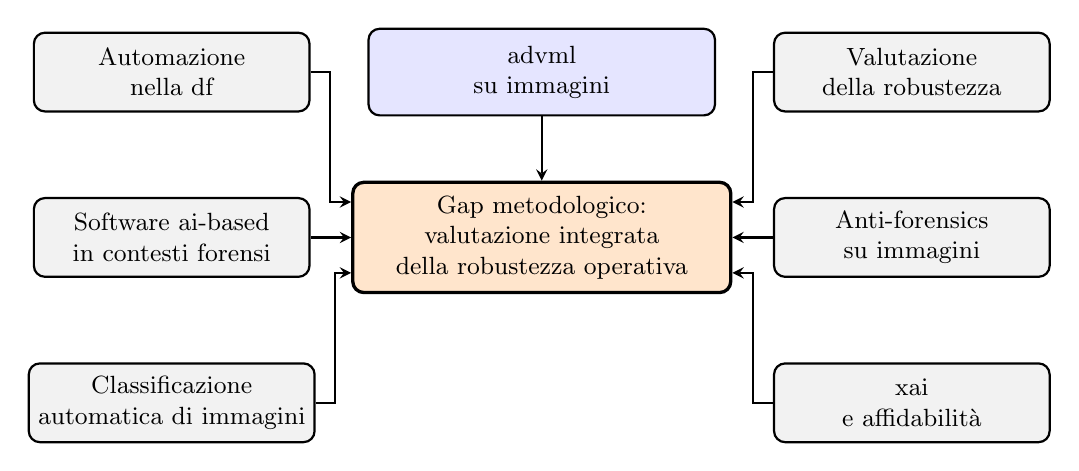
\begin{tikzpicture}[
    every node/.style={font=\small, align=center},
    field/.style={
        rectangle, rounded corners,
        draw=black, thick,
        fill=gray!10,
        minimum width=3.5cm,
        minimum height=1.0cm
    },
    central/.style={
        rectangle, rounded corners,
        draw=black, thick,
        fill=blue!10,
        minimum width=4.4cm,
        minimum height=1.1cm
    },
    gap/.style={
        rectangle, rounded corners,
        draw=black, very thick,
        fill=orange!20,
        minimum width=4.8cm,
        minimum height=1.4cm
    },
    arrow/.style={->, thick, >=stealth}
]

% Riga superiore
\node[field]   (ai_df)      at (0,   5.8) {Automazione\\nella \gls{df}};
\node[central] (advml)      at (4.7, 5.8) {\gls{advml}\\su immagini};
\node[field]   (robustness) at (9.4, 5.8) {Valutazione\\della robustezza};

% Riga centrale
\node[field] (tools)         at (0,   3.7) {Software \gls{ai}-based\\in contesti forensi};
\node[gap]   (gap)           at (4.7, 3.7) {Gap metodologico:\\valutazione integrata\\della robustezza operativa};
\node[field] (antiforensics) at (9.4, 3.7) {Anti-forensics\\su immagini};

% Riga inferiore
\node[field] (classification) at (0,   1.6) {Classificazione\\automatica di immagini};
\node[field] (xai)            at (9.4, 1.6) {\gls{xai}\\e affidabilità};

% Punti distinti di ingresso sul box gap
\coordinate (gapNW) at ([yshift=0.45cm]gap.west);
\coordinate (gapW)  at (gap.west);
\coordinate (gapSW) at ([yshift=-0.45cm]gap.west);

\coordinate (gapNE) at ([yshift=0.45cm]gap.east);
\coordinate (gapE)  at (gap.east);
\coordinate (gapSE) at ([yshift=-0.45cm]gap.east);



% Frecce da sinistra verso il gap
\draw[arrow] (ai_df.east)          -- ++(0.25,0) |- (gapNW);
\draw[arrow] (tools.east)          -- (gapW);
\draw[arrow] (classification.east) -- ++(0.25,0) |- (gapSW);

% Frecce da destra verso il gap
\draw[arrow] (robustness.west)     -- ++(-0.25,0) |- (gapNE);
\draw[arrow] (antiforensics.west)  -- (gapE);
\draw[arrow] (xai.west)            -- ++(-0.25,0) |- (gapSE);


% Freccia centrale
\draw[arrow] (advml.south) -- (gap.north);

\end{tikzpicture}

\caption{Strutturazione dei principali filoni della letteratura rispetto al gap metodologico affrontato dalla presente tesi.}
\label{fig:sota-literature-gap}
\end{figure}




Il gap specifico individuato dalla presente tesi riguarda quindi la limitata disponibilità di protocolli sperimentali integrati che combinino, nello stesso disegno valutativo, classificazione automatizzata o recupero semantico di immagini, validazione \textit{human-in-the-loop} del dataset, modelli proxy eterogenei, software AI-based selezionati per la valutazione operativa in contesto forense, perturbazioni adversariali, trasformazioni anti-forensi, metriche quantitative e analisi spiegabile del comportamento dei modelli. La rilevanza di tale integrazione deriva dal fatto che, in un contesto forense, l'affidabilità di un sistema automatico non può essere valutata soltanto come proprietà isolata del classificatore. Essa dipende anche dalla qualità e dalla rappresentatività dei dati, dalla presenza di casi borderline o fuori distribuzione, dalla natura delle manipolazioni applicate, dalla trasparenza del software impiegato e dall'effetto che eventuali errori possono produrre sul triage e sulla selezione delle evidenze.

La presente tesi si colloca precisamente in questa lacuna. Il suo contributo consiste nel condurre una valutazione sperimentale della robustezza operativa di modelli proxy e software AI-based impiegati, nel contesto della \gls{df}, per la classificazione automatizzata o il recupero semantico di immagini di potenziale interesse investigativo, considerando congiuntamente la dimensione algoritmica e quella operativo-investigativa. L'obiettivo non è soltanto misurare il degrado prestazionale in condizioni avverse, ma comprendere come tale degrado possa incidere sulla capacità del sistema di supportare l'analista nella selezione di contenuti rilevanti. In questa prospettiva, la robustezza viene trattata non come attributo astratto del modello, ma come requisito funzionale per l'uso controllato dell'\gls{ai} nei workflow di \gls{df}.

Il posizionamento della tesi è dunque duplice. Da un lato, essa si collega alla letteratura sull'\gls{advml}, sulla valutazione della robustezza e sull'\gls{xai}, assumendo che i sistemi di classificazione debbano essere valutati anche in presenza di input ostili, degradati o anomali. Dall'altro, si colloca nel dominio della \gls{df}, dove la qualità dell'automazione deve essere giudicata rispetto alla sua utilità operativa, alla verificabilità dei risultati e alla possibilità di mantenere il controllo umano sul processo di analisi. Questa impostazione consente di superare una valutazione puramente prestazionale e di affrontare il problema della robustezza come questione metodologica, tecnica e forense. Tale spazio di ricerca motiva il protocollo sperimentale \gls{fairlab}, adottato nella presente tesi e descritto nel capitolo successivo.